\documentclass{standalone}
\usepackage{hsbcommon}
%% Show/hide steps for standalone work — edit this line:
\makeatletter\AtBeginDocument{\@buildstepset{2}}\makeatother
\usepackage{tikz}
\begin{document}
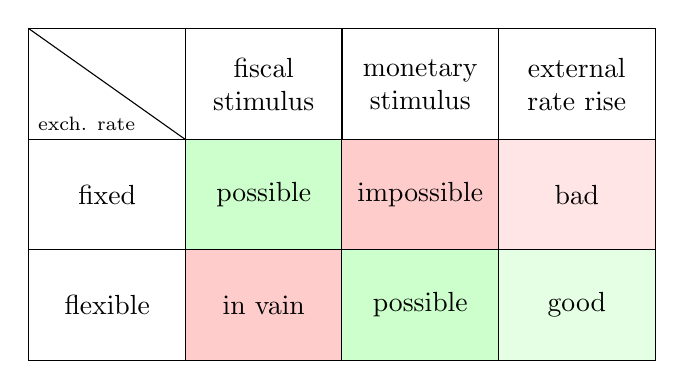
\begin{tikzpicture}
\tikzset{
    firstrow/.style={
        draw,
        text width=50pt,
        minimum height=40pt,
        align=center,
        anchor=west,
        xshift=-0.5pt
    },
    row/.style={
        draw,
        text width=50pt,
        minimum height=40pt,
        align=center,
        anchor=north,
        yshift=0.5pt
    },
    allrow/.style={
        draw,
        text width=50pt,
        minimum height=80pt,
        align=center,
        anchor=north,
        yshift=0.5pt  
    }
}
    
    \node[firstrow] (a0) at (0,0)     {};
    \draw (a0.north west) -- (a0.south east);
    \node[above right] at (a0.south west) {\scriptsize exch. rate};
    
    \node[firstrow] (a1) at (a0.east) {fiscal stimulus};
    \node[firstrow] (a2) at (a1.east) {monetary stimulus};
    \node[firstrow] (a3) at (a2.east) {external rate rise};

    \node[row] (b0) at (a0.south) {fixed};
    \node[row] (c0) at (b0.south) {flexible};
    \ifstep{1}{
        \node[allrow] (b1) at (a1.south) {$IS\rightarrow$} ;
        \node[allrow] (b2) at (a2.south) {$LM\rightarrow$} ;
        \node[allrow] (b3) at (a3.south) {$ZZ\uparrow$};
        

    }
    \ifstep{2}{
        \node[row,fill=green!20] (b1) at (a1.south) {possible};
        \node[row,fill=red!20] (b2) at (a2.south) {impossible};
        \node[row,fill=red!10] (b3) at (a3.south) {bad};
        
        \node[row,fill=red!20] (c1) at (b1.south) {in vain};
        \node[row,fill=green!20] (c2) at (b2.south) {possible};
        \node[row,fill=green!10] (c3) at (b3.south) {good};
    }
    
\end{tikzpicture}

\end{document}

\begin{frame}{Findings: Overview}
\mytable{
        \newcommand\exports{\text{Ex}}
        \begin{tabular}{c||c|c|c}
             Exch. Rate  & Monetary Policy & Fiscal Policy & Foreign Policy\\ 
             Regime  & $\Delta i <0$ & $\Delta G >0$ & $\Delta i_{int} >0$ \\ 
             & LM shifts right & IS shifts right  & ZZ shifts up\\
             \hline\hline
             % flexible & \textbf{affects GDP}  & primary effect & $\Delta Exp > 0$ \\
            flexible     & depreciation & appreciation & depreciation \\  
                 &  $\Delta \exports >0$ & $\Delta \exports <0$ & $\Delta \exports >0$\\
                 & & offset & $IS$ shifts right\\
                & $\rightarrow$ effect & no effect & pos. effect\\
             \hline
             fixed & no depreciation  & no appreciation & no depreciation \\
              & buy home curr. & sell home curr. & buy home curr. \\
              & (contradiction) & $\rightarrow$ & $\rightarrow$ \\
              &  & $LM$ shifts right & $LM$ shifts left\\
              & & $\rightarrow$ effect & neg. effect \\
        \end{tabular}
}
\end{frame}